\begin{enumerate}[A]
	\item 轴的受力分析
	\begin{enumerate}[a]
		\item 画受力简图
		\par 圆周力 $F_{t1}=1215.44$,$F_{t2}=2598.99$ \\
		径向力 $F_{\r1}=442.38$,$F_{r2}=945.95$
		\item 计算支反力 
		\begin{figure}[H]
			\begin{center}
				\caption{轴\uppercase\expandafter{\romannumeral2}的支反力图}
				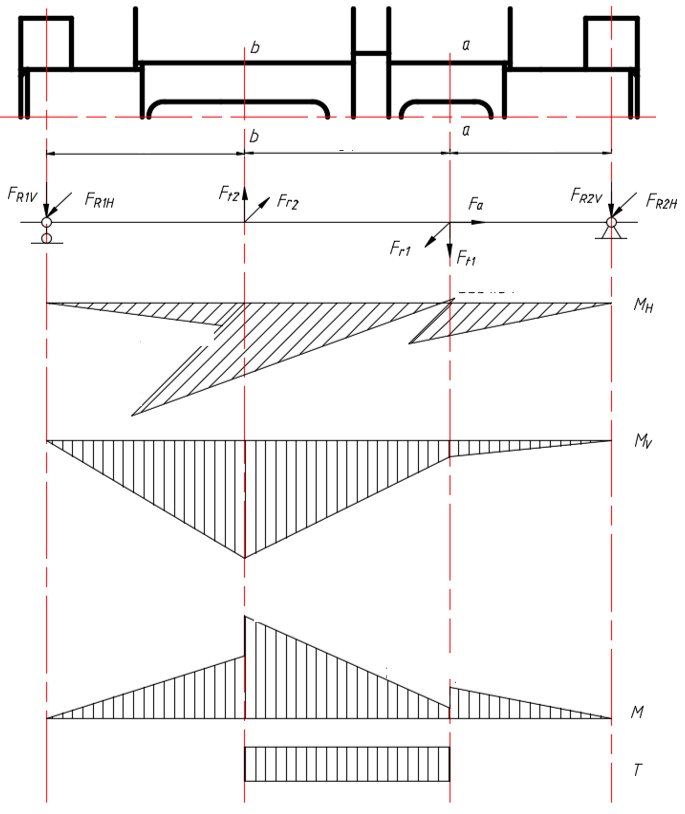
\includegraphics[width=0.8\textwidth]{pic/jiaohe2.png}
			\end{center}
		\end{figure}
		\par 在水平面上:
		$$F_{R1H}=\dfrac{F_{r2}\cdot \left(B_2+C_2\right)-F_{r1}\cdot C_2-F_a\cdot \dfrac{d}{2}}{A_2+B_2+C_2}=439.20$$
		$$F_{R2H}=F_{r2}-F_{r1}-F_{R1H}=64.37$$
		\par 在垂直平面上:
		$$F_{R1V}=\dfrac{F_{t2}\cdot \left(B_2+C_2\right)-F_{t1}\cdot C_2}{A_2+B_2+C_2}=1206.71$$
		$$F_{R2V}=F_{t2}-F_F_{t2}-F_{R1V}=176.84$$
		轴承1的总的支反力为
		$$F_{R1}=\sqrt{{F_{R1H}}^2+{F_{R1V}}^2}=1284.15$$
		轴承2的总的支反力为
		$$F_{R2}=\sqrt{{F_{R2H}}^2+{F_{R2V}}^2}=188.19$$
		\item 画弯矩图
		\par 在水平面上 \\
		a-a剖面线左侧\\
		$$M_{aH}=F_{R1H}\left(A_2+B_2\right)-F_{R2}B_2=43482.825$$
		a-a剖面右侧 \\
		$$M^{\prime}_{aH}=F_{R2H}C_2=3710.275$$
		b-b剖面线左侧\\
		$$M_{bH}=F_{R1H}A_2=30304.8$$
		b-b剖面右侧 \\
		$$M^{\prime}_{bH}=F_{R2H}\left(B_2+C_2\right)+F_{R1}B_2=77798.575$$
		垂直面上,a-a剖面
		$$M_{aV}=F_{R2V}C_2=10168.3$$
		b-b剖面
		$$M_{bV}=F_{R2V}A_2=83262.99$$
		合成弯矩\\
		a-a剖面左侧\\
		$$M_a=\sqrt{{M_{aH}}^2+{M_{aV}}^2}=44655.91$$
		a-a剖面右侧\\
		$$M^{\prime}_a=\sqrt{{M^{\prime}_{aH}}^2+{M_{aV}}^2}=10820.99$$
		b-b剖面左侧\\
		$$M_b=\sqrt{{M_{bH}}^2+{M_{bV}}^2}=88606.47$$
		b-b剖面右侧\\
		$$M^{\prime}_b=\sqrt{{M^{\prime}_{bH}}^2+{M_{bV}}^2}=113953.2526$$
		
		\item 画转矩图$$T=2.939\times 10^4$$
	\end{enumerate}
	\item 校核轴的强度
	\par b-b剖面右侧的弯曲强度大,有转矩,为危险截面。
	\par 该截面抗弯模量为
	$$W=0.1{d_2}^3-\dfrac{bt\left(d_2-t\right)^2}{2d_2}=3312,02$$
	该截面的抗扭截面模量为
	$$W_T=0.2{d_2}^3-\dfrac{bt\left(d_2-t\right)^2}{2d_2}=7342,42$$
	弯曲应力$$\sigma_b=\dfrac{M}{W}=34.41$$
	$$\sigma_a=\sigma_b=34.41$$
	$$\sigma_m=0$$
	扭剪应力
	$$\tau_T=\dfrac{T}{W_T}=4.06$$
	$$\tau_a=\tau_m=\dfrac{\tau_T}{2}=2.03$$
	\par 调质处理的45钢,由参考文献\cite{2}表9.3可以查得$\sigma_b=650$,$\sigma_{-1}=300$,$\tau_{-1}=155$;材料等效系数$\psi_\sigma=0.2$,$\psi_\tau=0.1$。
	\par 轴由两个键槽,取$K_\sigma=1.83$,$K_\tau=1.63$。
	\par 查参考文献\cite{2}表9.12得$\epsilon_\sigma=0.88$,$\epsilon_\tau=0.81$。
	\par 查参考文献\cite{2}表9.9得$\beta=1$。
	\par 由此,安全系数计算如下:
	$$S_\sigma=\dfrac{\sigma_{-1}}{\dfrac{K_\sigma}{\beta \epsilon_\sigma}\sigma_a+\psi_\sigma \sigma_m}=4.19$$
	$$S_\tau=\dfrac{\tau_{-1}}{\dfrac{K_\tau}{\beta \epsilon_\tau}\tau_a+\psi_\tau \tau_m}=36.14$$
	$$S=\dfrac{S_\sigma\cdot S_\tau}{\sqrt{{S_\sigma}^2+{S_\tau}^2}}=4.16$$
	\par 由参考文献\cite{2}表9.13得许用安全系数$\left[S\right]=1.3\sim 1.5$,显然$S>\left[S\right]$,故a-a截面安全。
	
	\item 校核键连接的强度
	\par 键连接的挤压应力\\$$\sigma_p=\dfrac{4T}{dhl}$$
	式中:d——键连接处的轴径,mm;\\
	T——传递的转矩,N·mm;\\
	h——键的高度,mm;\\
	l——键连接长度,mm;
	\par 故大齿轮处键连接的挤压应力为$$\sigma_p=\dfrac{4T}{dhl}=56.13$$小齿轮处键连接的挤压应力为$$\sigma_p=\dfrac{4T}{dhl}=21.96$$
	\par 键、轴材料均为45钢,$\left[\sigma_p\right]= 120~150$。$\sigma_p<\left[\sigma_p\right]$,故强度满足需要。
	\item 校核轴承强度
	\par 由参考文献\cite{1}表12.4查得6205轴承的$C_r=14000$,$C_0=7880$。
	\begin{enumerate}[a]
		\item 计算轴承的轴向力
		\par 由于是深沟球轴承和圆柱齿轮,所以轴向力不予考虑。所以需要同时校核轴承1和2。
		\item 计算当量动载荷
		\par 由于是深沟球轴承和圆柱齿轮,所以无需计算当量动载荷,只需计算轴承寿命。
		\item 校核轴承寿命
		\begin{itemize}
			\item 校核轴承1的寿命
			\par 轴承在\SI{100}{\degreeCelsius}下工作,$f_T=1$。根据其载荷性质,取$f_F=1.2$。
			\par 轴承寿命为
			$$L_h=\dfrac{10^6}{60n_{\mathrm{\uppercase\expandafter{\romannumeral2}}}}{\left(\dfrac{f_tC_r}{f_FF_1}\right)}^3=43126.4265$$
			\par 已知减速器使用年限为五年两班工作制,则预期寿命为
			$${L_h}^{\prime}=8\times 2\times 250\times 5=20000$$
			故轴承的寿命很充裕
			\item 校核轴承2的寿命
			\par 轴承在\SI{100}{\degreeCelsius}下工作,$f_T=1$。根据其载荷性质,取$f_F=1.2$。
			\par 轴承寿命为
			$$L_h=\dfrac{10^6}{60n_{\mathrm{\uppercase\expandafter{\romannumeral2}}}}{\left(\dfrac{f_tC_r}{f_FF_1}\right)}^3=13702541.01$$
			\par 已知减速器使用年限为五年两班工作制,则预期寿命为
			$${L_h}^{\prime}=8\times 2\times 250\times 5=20000$$
			故轴承的寿命很充裕
		\end{itemize}
	\end{enumerate}
\end{enumerate}